\documentclass{egpubl}
\usepackage{eg2017}

\Poster      % uncomment for (final) Short Conference Presentation

\electronicVersion % can be used both for the printed and electronic version

\ifpdf \usepackage[pdftex]{graphicx} \pdfcompresslevel=9
\else \usepackage[dvips]{graphicx} \fi

\PrintedOrElectronic

% prepare for electronic version of your document
\usepackage{t1enc,dfadobe}

\usepackage{egweblnk}
\usepackage{cite}

%%% Added packages and commands %%%
\usepackage[usenames,dvipsnames]{xcolor}
\usepackage{amsmath}
\usepackage{amssymb}

\newcommand{\added}[1]{{\color{Red}\textbf{#1}}} % do not need this probably
\newcommand{\note}[3]{{\color{#2}\textbf{#1: #3}}}
\newcommand{\henrik}[1]{\note{HENRIK}{WildStrawberry}{#1}}
\newcommand{\john}[1]{\note{JohnKa}{RubineRed}{#1}}
\newcommand{\unsure}[1]{\note{USIKKER}{Green}{#1}}
\newcommand{\IGNORE}[1]{}
\graphicspath{{fig/}}

% correct bad hyphenation here
\hyphenation{to-po-lo-gi-cal-ly to-po-lo-gy      ini-tial  col-our pat-ches}

\title[Non-rectangular gradient mesh tool]
{A Gradient Mesh Tool for Non-Rectangular Gradients}

% for anonymous conference submission please enter your SUBMISSION ID
% instead of the author's name (and leave the affiliation blank) !!
\author[poster]
{\parbox{\textwidth}{\centering poster}
	\\
	% School/Institution here (if accepted)
	{\parbox{\textwidth}{\centering } }
}

% if the Editors-in-Chief have given you the data, you may uncomment
% the following five lines and insert it here
%
% \volume{27}   % the volume in which the issue will be published;
% \issue{1}     % the issue number of the publication
% \pStartPage{1}      % set starting page

\begin{document}
	
	% \teaser{
	%  \includegraphics[width=\linewidth]{eg_new}
	%  \centering
	%   \caption{New EG Logo}
	% \label{fig:teaser}
	% }
	
	\maketitle
	
	\begin{abstract}
		The gradient mesh tool, implemented in vector graphics software like Adobe Illustrator, is a popular tool for creating and manipulating complex colour gradients. The mesh-based tool is restricted to rectangular control meshes, making it hard for the user to work with more complicated shapes such as shapes with holes. We propose a new gradient mesh tool that supports non-rectangular control meshes, with native support for a wide range of different shapes. A user study indicates that our tool is easier to use in the setting of drawing colour gradients inside complicated shapes with holes.
		
		\begin{classification} % according to http:http://www.acm.org/about/class/1998
			\CCScat{Computer Graphics}{I.3.4}{Graphics Utilities}{Paint systems}
		\end{classification}
		
	\end{abstract}
	
	\section{Introduction}
	\label{sec:intro}
	
	In vector graphics design, working with complex colour functions is challenging. The restrictions of the linear gradient tool is one reason designers turn to pixel-based tools, like Adobe Photoshop, when the design turns complicated. This issue has been acknowledged in the research community and a wide range of different approaches have been proposed to make the design of colour gradients more effortless \cite{Orzan:2008,Lopez-Moreno:2013, Vergne:2012, Shao:2012}.
	
	The gradient mesh tool, found in vector graphics packages like Adobe Illustrator, Corel CorelDraw and Inkspace, is a popular tool for complex colour gradient design. It is useful in scenarios where the linear gradient tool does not suffice. However, it does not support non-rectangular gradients: the control mesh which the user interacts with must be of rectangular topology. In this paper, we propose a new tool for gradient mesh editing where the user can create and manipulate non-rectangular colour gradients, like the one shown in Fig.[REF-teaser]. Our approach takes advantage of a recent gradient mesh interpolation technique that supports arbitrary mesh topology~\cite{Lieng:2016}. Being able to model non-rectangular gradient meshes provides significant practical advantages, especially for vector shapes with holes.
	
%	\begin{figure}
%		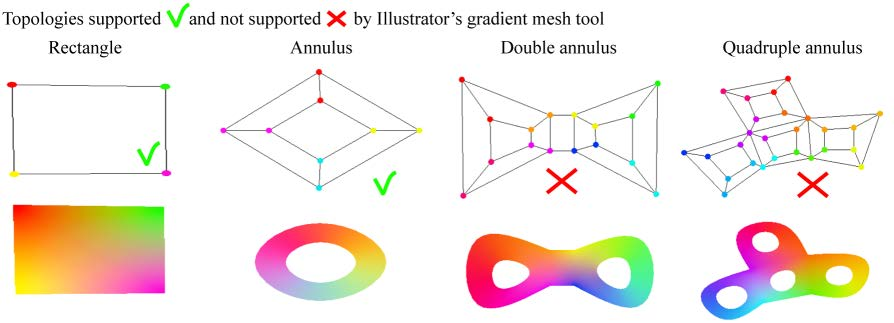
\includegraphics[]{illustratorVsOur.jpg}
%		\caption{Caption... Image courtesy of Lieng et al. \cite{Lieng:2016}}
%		\john{Should we use a new image, or is it OK to refer to the article and alter some of the original caption?}
%		\label{fig:IllustratorVsOur}
%	\end{figure}
	
	\section{Problem description}
	\label{sec:overview}
	
	In previous gradient mesh tools there are two approaches to mesh creation. The first option converts a vector graphics object compatible with rectangular gradient (i.e. a vector shape without holes) to a grid of control points. The user is required to input the number of rows and columns of the gradient mesh. The creation is dependent on a grid representation, and is therefore incompatible with non-rectangular gradient meshes.
	
	The second option is a point-and-click interface where the user clicks on a location inside the target shape and a new control point is created at the clicked location. This is attractive as the creation operation is independent from the underlying data structure and can give rise to several interpretations. However, the interaction produces a global alteration: when a control point is added, a new row and column is added to the entire mesh. It is therefore challenging to achieve local gradient edits and the user must consequently plan the structure of the mesh so that the number of rows and columns is kept to a minimum. In the non-rectangular setting, this would be even more challenging. Fig.~\ref{fig:adHocPentagon} illustrates a point-and-click interaction inside a polygon adjacent to a pentagon. The effect of such an interaction is ambiguous and any solution would be ad-hoc.
	
%	In conclusion, the user interaction already supported by the gradient mesh tool is hard to extend to the more flexible setting of non-rectangular control meshes.
	
	\begin{figure}[t]
		\centering
		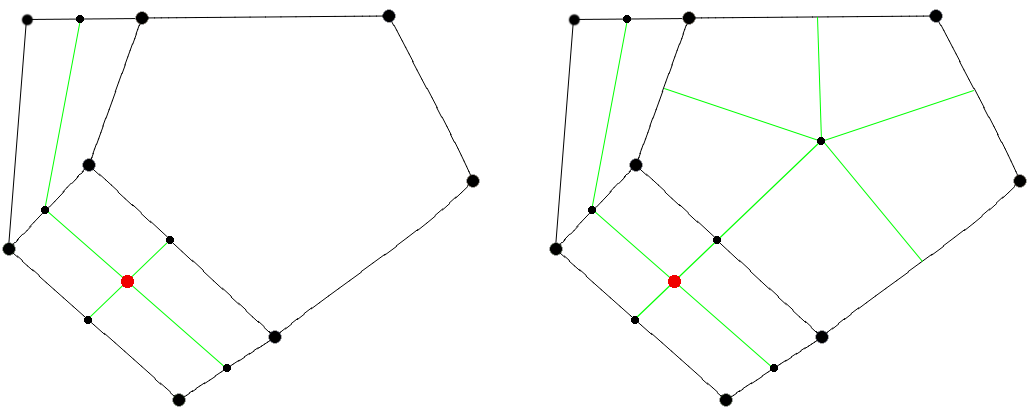
\includegraphics[scale=0.2]{pentagonCombined.png}
		\caption{The current point-and-click interface gives rise to ambiguous cases for irregular meshes. A new vertex is inserted at the location where the user clicks (red point). New edges are inserted from this point (green edges). The two control meshes show two possible solutions for mesh alteration at the irregular face (the pentagon). Both options give rise to a poor mesh quality (a T-junction and a high-valence vertex).
		}
		\label{fig:adHocPentagon}
	\end{figure}
	
	\section{A tool for creating non-rectangular gradient meshes}
	\label{sec:method}
	
	Our approach takes inspiration from the pen tool found in SketchUp. Our tool provide operations such as edge split and face deletion. Code and a demonstration video of the tool will be made available upon publication.
	
	In the following, we describe typical interactions with our tool to create and refine gradient meshes. The user create initial meshes \textit{face-by-face}, which can later be refined and manipulated. Our \textbf{line tool} enables the user to create single polygonal faces of arbitrary topology. The mesh is expanded by iteratively adding faces to it. To add a face, the user selects an existing mesh vertex and place new control points on the canvas. The face is closed by clicking on an existing mesh vertex. If the initial vertex closes the face, a non-manifold mesh can be achieved as shown in Fig.~\ref{fig:nonManifoldHoleMesh}.
	
	The user can further locally edit and refine the control mesh. The \textbf{edge split tool} splits a selected edge into two pieces. The inserted control point should then be connected to another mesh point to avoid valence-2 control points. Note that edges are modelled as cubic Bezier curves: each control point is associated with a gradient constraint for each of its edges that control the local influence of the colour of the control point. Such gradient constraints is a standard feature of gradient meshes. To ensure that the curve of the edge is maintained when the edge is split, the position of new control points are calculated using De Casteljau's algorithm. Finally, adjacent edges can be collapsed for mesh simplification and faces can be removed to introduce holes (Fig.~\ref{fig:nonManifoldHoleMesh}). We also support alterations at finer levels, using the multi-resolution adjustments of Lieng et al. \cite{Lieng:2016}.
	
%	\unsure{As previously mentioned, we employ the method of Lieng et al.~\cite{Lieng:2016} as the underlying interpolation technique. This method employs subdivision surfaces and supports the feature of multi-resolution mesh manipulation; that is, mesh alteration on different level of detail. TODO:Write why this is good, maybe colour points if good results}
	
	\begin{figure}[t]
		\centering
		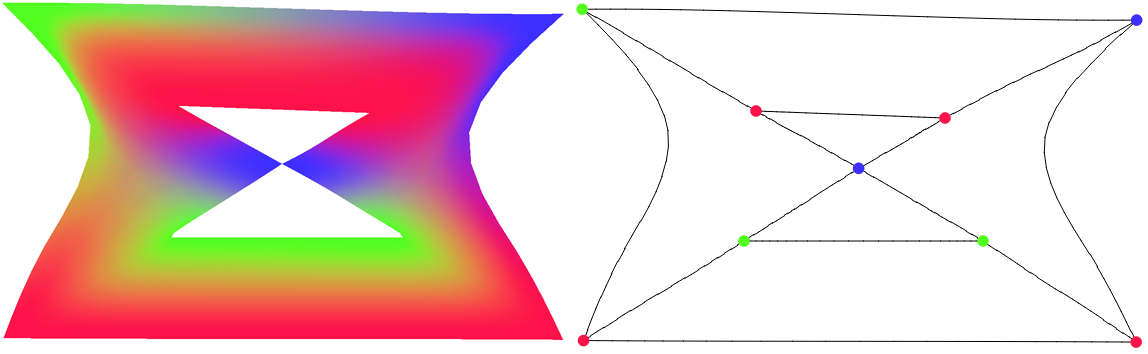
\includegraphics[scale=0.2]{HoleAndNonManifoldMesh.png}
		\caption{A non-manifold mesh with internal holes. Top: Faces are added iteratively. Bottom left: The inner faces have been removed.  Bottom right: The control mesh.}
		\label{fig:nonManifoldHoleMesh}
	\end{figure}
	
	\section{Informal user study}
	\label{sec:results}
	
	
%	Our tool was implemented in C++ with use of the libraries Qt (\url{https://www.qt.io/}) and OpenMesh (\url{http://www.openmesh.org/}). OpenMesh provides an generic and efficient way to store the mesh with the half-edge data structure, which supports arbitrary topology. The mesh is interpolated by employing the technique of Lieng et. al-~\cite{Lieng:2016}, as previously mentioned~\ref{sec:intro}. \john{Ha med mer her? Skrive om?}
	
	We preformed an informal user study where five subjects were tested: two professional designers and three art students. The subjects were given two task (creating one baseline rectangular mesh and one non-rectangular mesh), each completed with our tool and with Adobe Illustrator's gradient mesh tool. The tests were complemented with an user survey. The full results of the study will be made publicly available. For the baseline test, all subjects were able to create a regular mesh. The data from this test suggest that Adobe Illustrator either provides a generally better user interface (with operations like undo) or because users are already familiar with Illustrator it is easier for them to work with it over our tool. For the non-regular mesh, users preferred our tool over Illustrator's. The subjects praised our tool for enabling face-specific manipulation capabilities such as face deletion.
	
	\section{Future work}
	\label{sec:FW}
	
	Though our gradient mesh tool offers opportunities to work with non-rectangular gradient meshes, it is not an full experience graphical design software application. In the future, we aim to rewrite our tool as a plug-in for Adobe Illustrator. This presents several issues, as the underlying mesh representation in Illustrator differs from ours. One approach can be to incorporate Pixar's OpenSubdiv library with Illustrator's SDK.
	
	\bibliographystyle{eg-alpha}
	
	\bibliography{refs}
	
\end{document}